\section{Rewards and collectables}
One of the main components of Sophie's Flying Castle game is finding collectibles throughout the world.
Collectibles are items that are required to be collected in order to achieve 100\%
completion of the game, but they are not compulsorily required to go on in the main storyline. Collectibles, along with coins and crafting materials, are the fundamental part of the reward system of the game; in fact they constitute the prizes for any successful in-game action of the player. Moreover they even grant rewards to all the players who will deeply explore the maps, reaching high percentages of completion of the game.\\

There are three category of collectibles:
\begin{enumerate}
\item \textbf{Hats}: these objects can be hats, wigs and helmets. If they are worn they provide skill bonuses during the game wherever Sophie is, as long as she keeps them on.
\item \textbf{Lanterns}: these objects work as weapons for Sophie. They contain Calcifer and they are evolutions of the basic lantern, given to Sophie at the beginning of the story. While they are held by Sophie, they provide skill bonuses during the combat against enemies. 
\item \textbf{Clothes}: these objects are special clothes that Sophie may get during the game and they provide effects depending on where Sophie is.  
  \end{enumerate}

A player can only use one object per category at a time.

Example: if Sophie had unlocked two or more magic hats, she could still wear only one. But if she had unlocked also a magic lantern, she might wear a hat and hold the lantern.

Collectables can be sold for Difficulty * 10 coins at merchants' stands as well as crafting materials can be sold for half of their buying price at merchants' stands. Collectables can be bought back at the same stand where the player sold them for Difficulty * 20 in case they have been crafted or for the original selling price in case they have been bought (e.g. in case the player sold them by mistake).



\subsection{Level completion rewards}
These collectables are items that Sophie may obtain only by completing specific actions during the course of the main story and they can not be crafted or obtained in an other way.

%These are tied to a small reward in coins, materials or experience and bound to levels of Sophie's abilities.

%The player will receive these items just by playing the main story of the game.\\\\
%There are three category of rewards:
%\begin{enumerate}
%\item \textbf{Hats}\\
  {\small
\begin{longtable}[H]{|p{1.8cm}|p{1.5cm}|p{2cm}|p{2.6cm}|p{5.3cm}|p{1.2cm}|}
\hline
\multicolumn{6}{|c|}{\cellcolor[HTML]{656565}{\color[HTML]{FFFFFF} \textbf{Hats}}}  \\\hline
\multicolumn{1}{c|}{\cellcolor[HTML]{C0C0C0}\textbf{Name}} &
\cellcolor[HTML]{C0C0C0}{\color[HTML]{000000} \textbf{Image}} &
\multicolumn{1}{c|}{\cellcolor[HTML]{C0C0C0}{\color[HTML]{000000} \textbf{Level}}} &
\multicolumn{1}{c|}{\cellcolor[HTML]{C0C0C0}{\color[HTML]{000000} \textbf{Bonus}}} &
\multicolumn{1}{c|}{\cellcolor[HTML]{C0C0C0}{\color[HTML]{000000} \textbf{Brief description}}} &
\multicolumn{1}{c|}{\cellcolor[HTML]{C0C0C0}{\color[HTML]{000000} \textbf{Difficulty}}}\\\hline
\textbf{Derby} & \raisebox{-0.8\height}{\includegraphics[height=1.5cm]{Images/Hats/derby}} & First Steps &
\begin{tabular}[c]{@{}l@{}} +1 Wisdom \\ \end{tabular}
& Sophie is getting it in a tutorial level where she learns how to sew new hats & 0 \\\hline
\textbf{Balmoral bonnet} & \raisebox{-0.8\height}{\includegraphics[height=1.5cm]{Images/Hats/balmoralBonnet}} & In enemy territory &
\begin{tabular}[c]{@{}l@{}} +1 TAC0 \\ +1 Intelligence \\ +1 Constitution\\ -1 AC\end{tabular}  &
Sophie will get it only if she chooses to bypass the Captain in the Castle of Dynamia and she solves the puzzle & 5 \\\hline
\textbf{Suliman's hat} & \raisebox{-0.8\height}{\includegraphics[height=1.5cm]{Images/Hats/suliman}} & Nasty surprise(s) &
\begin{tabular}[c]{@{}l@{}} +2 Wisdom \\ +2 Charisma \\ +3 TAC0\end{tabular} & Sophie gets it by speaking with Suliman & 3 \\\hline
\textbf{Winged helmet} & \raisebox{-0.8\height}{\includegraphics[height=1.5cm]{Images/Hats/helmetWings}} & The djinn of the desert &
\begin{tabular}[c]{@{}l@{}} +3 TAC0 \\ +2 Intelligence \\ +3 Constitution\end{tabular}  &
Sophie gets it in when she drives the flying castle for the first time & 0 \\\hline
\textbf{Desert} & \raisebox{-0.8\height}{\includegraphics[height=1.5cm]{Images/Hats/desert}} & The djinn of the desert &
\begin{tabular}[c]{@{}l@{}} +3 Intelligence\\ -2 Charisma \\ -3 AC\\  +4 Constitution\\ \end{tabular} &
Sophie can give Belzel some of her crafting materials in exchange for this & 2 \\\hline
\textbf{Panter} & \raisebox{-0.8\height}{\includegraphics[height=1.5cm]{Images/Hats/panter}} & The spirits realm &
\begin{tabular}[c]{@{}l@{}} +5 Constitution \\ -2 AC \\ +4 Strength \end{tabular}
& Sophie gets it only if she chooses to bypass the Panther in the spirits realm and she solves the puzzle & 5 \\\hline
\textbf{Sultan of piety} & \raisebox{-0.8\height}{\includegraphics[height=1.5cm]{Images/Hats/sultanPiety}} &
Fire and secrets & \begin{tabular}[c]{@{}l@{}} +5 Intelligence \\ +5 Charisma \\ +3 Constitution \\ -1 AC \end{tabular} & Sophie will get it if she chooses to spare Mizar & 5 \\\hline
\textbf{Sultan of vengeance} & \raisebox{-0.8\height}{\includegraphics[height=1.5cm]{Images/Hats/sultanVengeance}} &
Fire and secrets & \begin{tabular}[c]{@{}l@{}} +6 Strength \\ +4 Dexterity \\ +3 Constitution \\ -2 AC \end{tabular} &
Sophie will get it if she chooses to defeat Mizar & 5 \\\hline    
\end{longtable}
}

%\item \textbf{Lanterns}\\
  {\small
\begin{longtable}[H]{|p{1.8cm}|p{1.5cm}|p{2cm}|p{2.6cm}|p{5.3cm}|p{1.2cm}|}
\multicolumn{6}{|c|}{\cellcolor[HTML]{656565}{\color[HTML]{FFFFFF} \textbf{Collectable}}}                                                 \\ \hline
\multicolumn{1}{c|}{\cellcolor[HTML]{C0C0C0}\textbf{Lanterns}} & \cellcolor[HTML]{C0C0C0}{\color[HTML]{000000} \textbf{Image}} &
\multicolumn{1}{c|}{\cellcolor[HTML]{C0C0C0}{\color[HTML]{000000} \textbf{Level}}} &
\multicolumn{1}{c|}{\cellcolor[HTML]{C0C0C0}{\color[HTML]{000000} \textbf{Damage}}} &
\multicolumn{1}{c|}{\cellcolor[HTML]{C0C0C0}{\color[HTML]{000000} \textbf{Brief description}}} &
\multicolumn{1}{c|}{\cellcolor[HTML]{C0C0C0}{\color[HTML]{000000} \textbf{Difficulty}}}\\\hline
\textbf{Magic lantern} & \raisebox{-0.8\height}{\includegraphics[height=1.5cm]{Images/Lanterns/basis}} & Where is Howl? & 1d8 &
Sophie is getting it before leaving to Dynamia. This is the basic weapon of Sophie. & 0\\ \hline
\textbf{Demonic} & \raisebox{-0.8\height}{\includegraphics[height=1.5cm]{Images/Lanterns/demonic}} & In enemy territory
& \begin{tabular}[c]{@{}l@{}} 1d10 \\ -2 Intelligence \\ +3 HP\end{tabular} &
Sophie will get it just if she chooses to fight the prisons boss in the castle of Dynamia and she defeats him.   & 5\\ \hline
%\textbf{} & & Nasty surprise(s) &  & \\ \hline
%\textbf{}  &  & Battle cry & & \\ \hline
%\textbf{} & & An ancient legend & &  \\ \hline
%\textbf{} &  & The djiin of the desert & & \\ \hline
%\textbf{} & & Nel blu dipinto di blu &  & \\ \hline
\textbf{Belzel's lantern} & \raisebox{-0.8\height}{
\includegraphics[height=1.5cm]{Images/Lanterns/belzel}} & The djinn of the desert &
\begin{tabular}[c]{@{}l@{}} 1d8 \\ +2 Strength \\ +4 HP\end{tabular}  &
Sophie may get it speaking with Belzel & 3\\ \hline
%\textbf{} &  & The spirits realm & & \\ \hline
%\textbf{} & & Fire and secrets & & \\ \hline
\textbf{Gold} & \raisebox{-0.8\height}{\includegraphics[height=1.5cm]{Images/Lanterns/gold}} & The spirits realm &
\begin{tabular}[c]{@{}l@{}} 1d10 \\ +4 Dexterity \\  +1 Wisdom \\ +1 AC \end{tabular} &
Sophie will get it only if she chooses to bypass a panter boss in the castle of Dynamia and she solves a puzzle & 5\\ \hline
\textbf{Five Hits} & \raisebox{-0.8\height}{\includegraphics[height=1.5cm]{Images/Lanterns/candelabrumFiveHits}} &
Fire and secrets  & \begin{tabular}[c]{@{}l@{}} 2d8 \\ +2 Dexterity \\ -2 AC \\ -4 HP \end{tabular} &
Sophie can get it if she chooses to spare Mizar. Sophie keeps it in her bag if she start the game a second time    & 5  \\ \hline
\textbf{Cristal} & \raisebox{-0.8\height}{\includegraphics[height=1.5cm]{Images/Lanterns/cristal}} & Fire and secrets
& \begin{tabular}[c]{@{}l@{}} 1d10 \\ -2 Strength \\ +3 Intelligence \\ -2 AC \\ +6 HP \end{tabular}
& Sophie can get if she chooses to defeat Mizar. Sophie keeps it in her bag if she start the game a second time & 5\\ \hline
\end{longtable}
}

%\item \textbf{Clothes}\\
  \begin{longtable}[H]{|p{2cm}|p{1.5cm}|p{2cm}|p{2.8cm}|p{6.3cm}|}
\hline
\multicolumn{5}{|c|}{\cellcolor[HTML]{656565}{\color[HTML]{FFFFFF} \textbf{Collectable}}}                                                                                                                                                                                                                                                                                                              \\ \hline
\multicolumn{1}{c|}{\cellcolor[HTML]{C0C0C0}\textbf{Clothes}} & \cellcolor[HTML]{C0C0C0}{\color[HTML]{000000} \textbf{Image}} & \multicolumn{1}{c|}{\cellcolor[HTML]{C0C0C0}\textbf{Levels}} & \multicolumn{1}{c|}{\cellcolor[HTML]{C0C0C0}{\color[HTML]{000000} \textbf{Bonus}}}    & \multicolumn{1}{c|}{\cellcolor[HTML]{C0C0C0}{\color[HTML]{000000} \textbf{Brief description}}}                                         \\ \hline
\textbf{Sophie's dress}& \raisebox{-0.8\height}{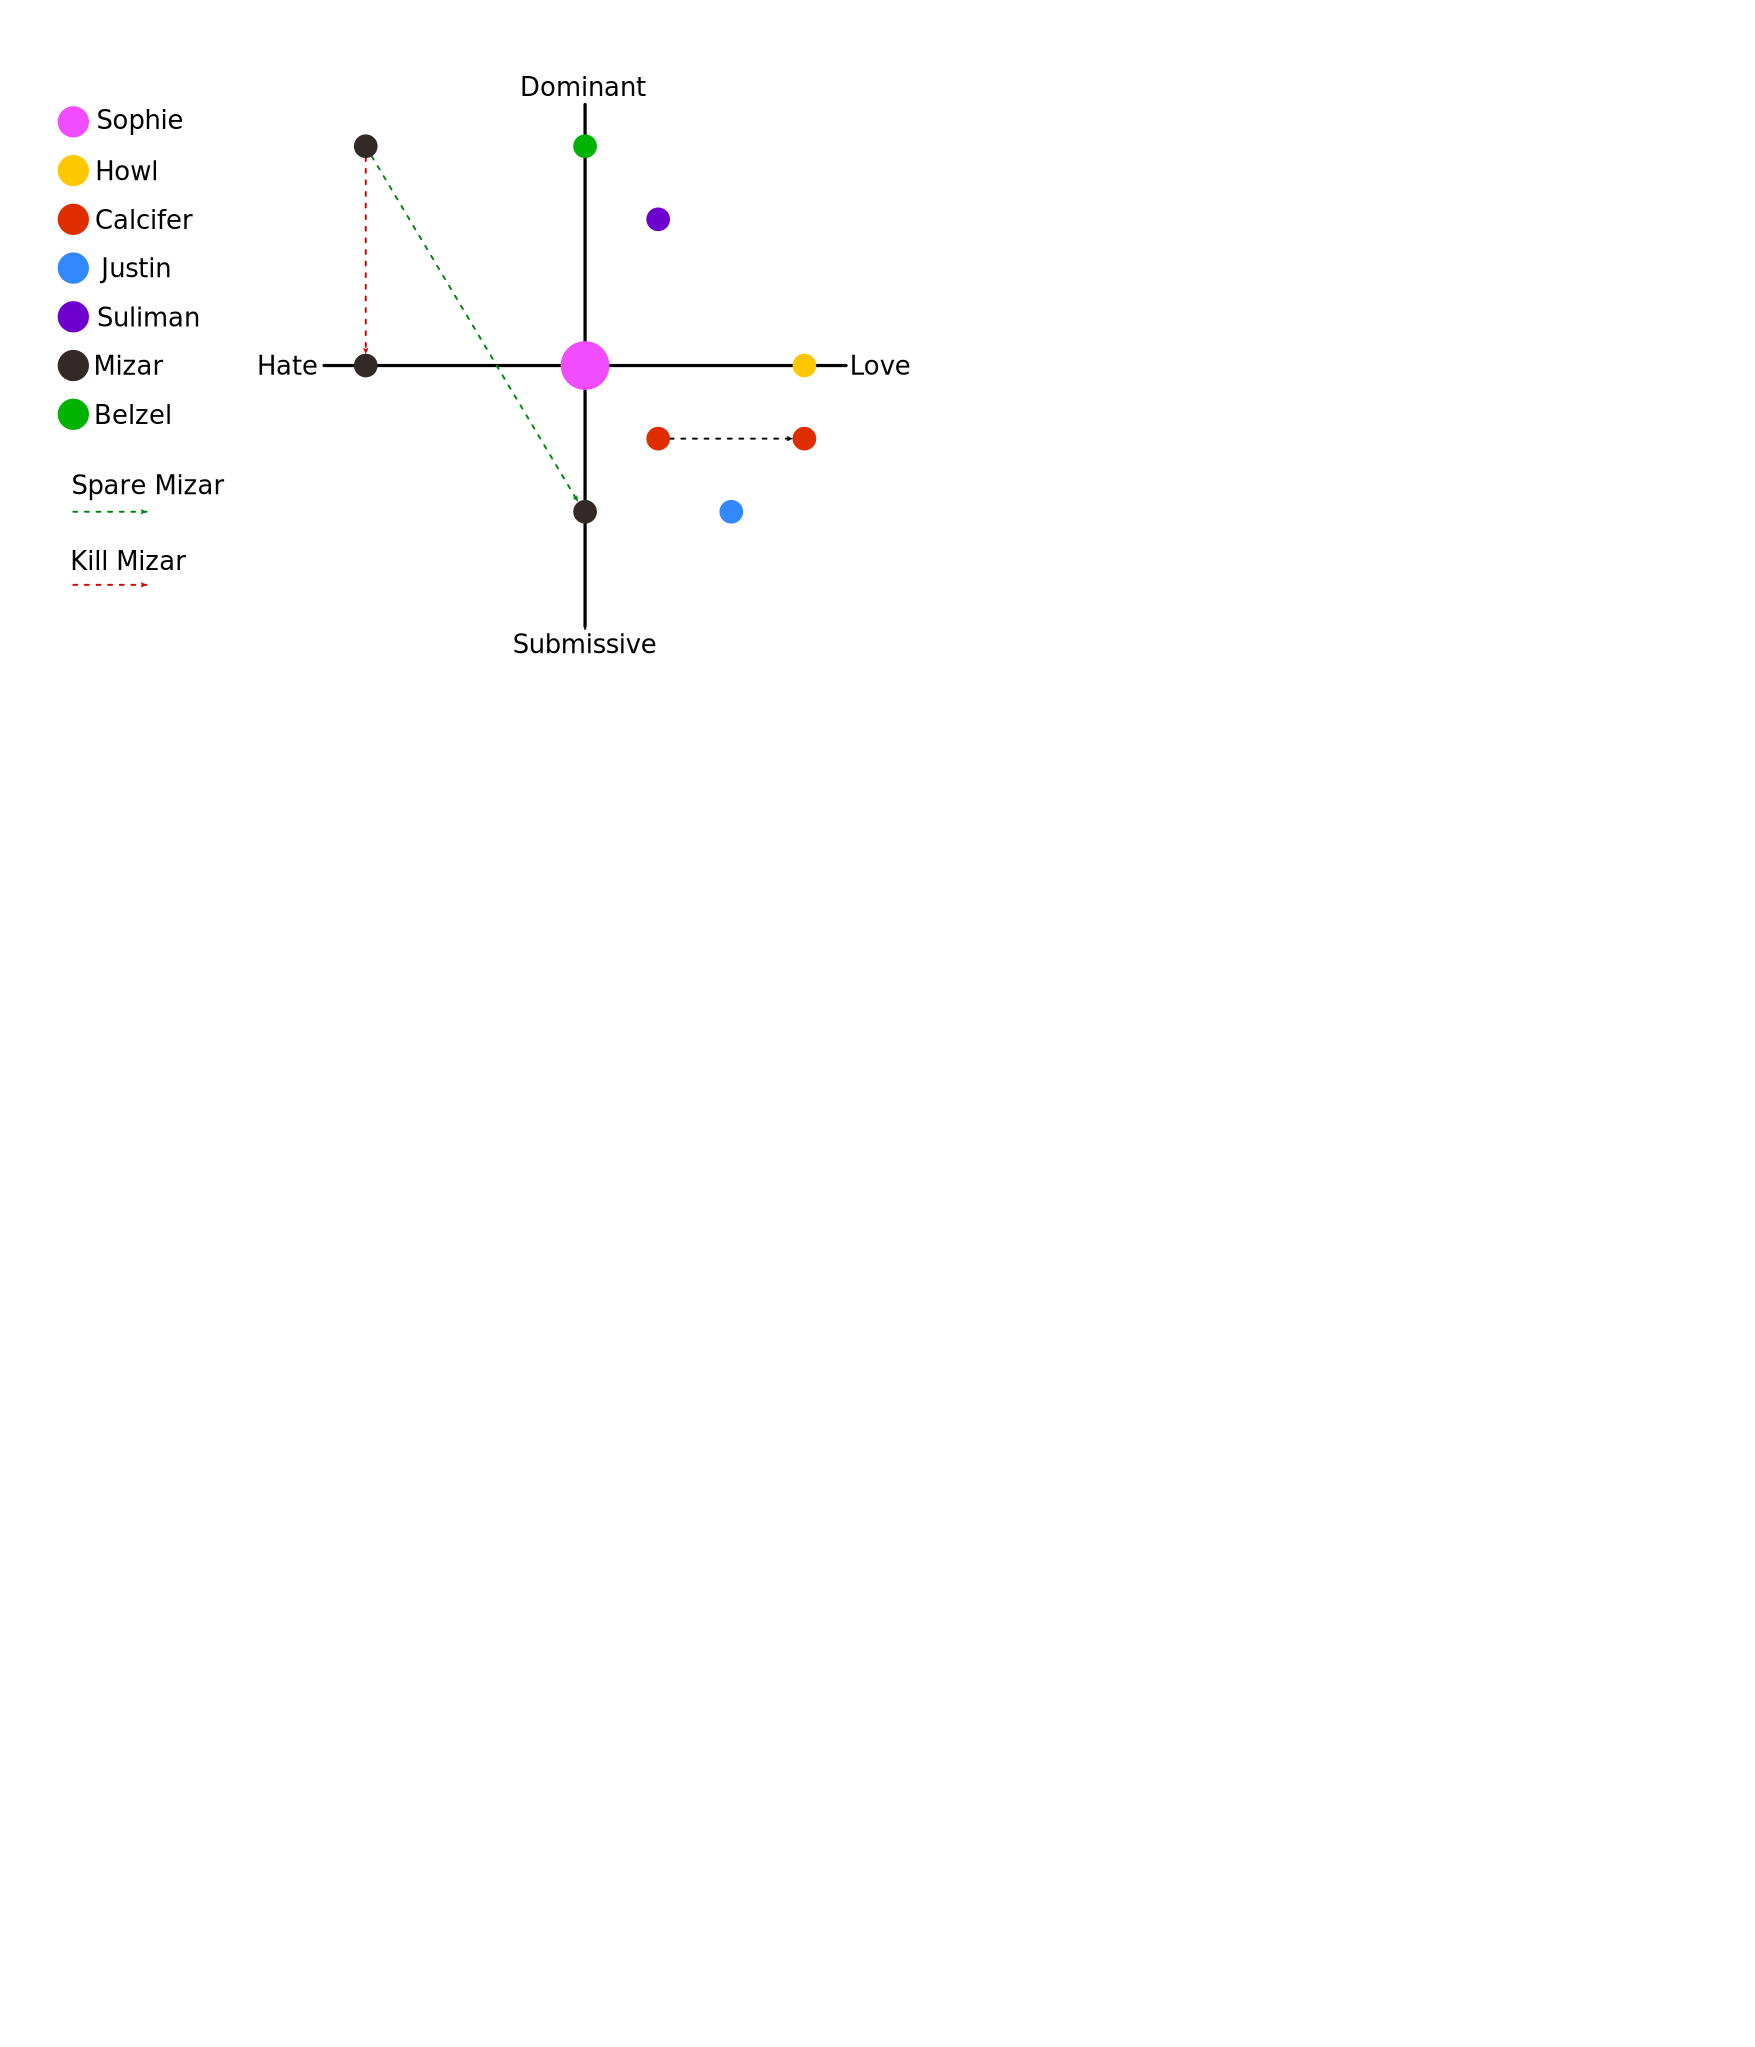
\includegraphics[height=1.5cm]{Images/Clothes/sophie}} & First steps & No bonus
& This is the Sophie's basic dress. \\ \hline
\textbf{Guard}& \raisebox{-0.8\height}{\includegraphics[height=1.5cm]{Images/Clothes/guards}} & The imprisoned friend & If the guards of Dynamia haven’t yet seen her, they take longer to spot her in Dynamia while
they are next to her. & Sophie can get it from a secondary mission in the Castle of Dynamia. She can follow a guard until he reaches a locker
room and take his clothes when he is gone. \\ \hline

\end{longtable}


%\end{enumerate}


\subsection{Others collectables and trophies}
These collectables are not related to the main story and the player could get them at anytime during the game. In order to receive them the player has to play the game deeply, exploring areas outside the ones he encountered during the main story flow, investing more time to get higher rewards.
%\begin{enumerate}
%\item \textbf{Hats}\\
  {\small
\begin{longtable}[H]{|p{1.8cm}|p{1.5cm}|p{2cm}|p{2.6cm}|p{5.3cm}|p{1.2cm}|}
\hline
\multicolumn{6}{|c|}{\cellcolor[HTML]{656565}{\color[HTML]{FFFFFF} \textbf{Collectable}}} \\\hline
\multicolumn{1}{c|}{\cellcolor[HTML]{C0C0C0}\textbf{Hats}} & \cellcolor[HTML]{C0C0C0}{\color[HTML]{000000} \textbf{Image}} &
\multicolumn{1}{c|}{\cellcolor[HTML]{C0C0C0}\textbf{Location}} &
\multicolumn{1}{c|}{\cellcolor[HTML]{C0C0C0}{\color[HTML]{000000} \textbf{Bonus}}} &
\multicolumn{1}{c|}{\cellcolor[HTML]{C0C0C0}{\color[HTML]{000000} \textbf{Brief description}}} &
\multicolumn{1}{c|}{\cellcolor[HTML]{C0C0C0}{\color[HTML]{000000} \textbf{Difficulty}}}\\\hline
\textbf{Winter} & \raisebox{-0.8\height}{\includegraphics[height=1.5cm]{Images/Hats/winter}} & Kingsbury &
\begin{tabular}[c]{@{}l@{}} +2 Wisdom\\ +2 Charisma \\ +2 HP\end{tabular} &
  Sophie can can find it in Kingsbury near the main place or sew it in the magic castle. They are required grey wool threads x10 and grey
  fabric x4& 3 \\\hline
  \textbf{Ascot cap} & \raisebox{-0.8\height}{\includegraphics[height=1.5cm]{Images/Hats/ascotCap}} & Dynamia / Flying castle &
  \begin{tabular}[c]{@{}l@{}} +2 Consitution\\ +2 Intelligence \\ +2 HP\end{tabular} & Sophie can can find it in
    Dynamia in the eastern part of the city or sew it in the magic castle.  It is required leather x20 & 1 \\\hline            
    \textbf{Shako} & \raisebox{-0.8\height}{\includegraphics[height=1.5cm]{Images/Hats/shako}} & Dynamia &
    \begin{tabular}[c]{@{}l@{}} +2 Strength\\ -4 Intelligence\\ -1 HP\end{tabular} &
      Shako hat is a trophy that Sophie can get if she defeats 30 guards in Dynamia.& 1 \\\hline
      %\textbf{Turban} & \raisebox{-0.8\height}{\includegraphics[height=1.5cm]{Images/Hats/turban}} & Dynamia
      %& \begin{tabular}[c]{@{}l@{}} +2 Dexterity \\ -2 TAC0 \end{tabular}  &
     % Sophie can find it in Dynamia it in the eastern part of the city. & 1 \\\hline
      \textbf{Baseball} & \raisebox{-0.8\height}{\includegraphics[height=1.5cm]{Images/Hats/baseball}} & Dynamia
      & \begin{tabular}[c]{@{}l@{}} +1 Constitution\\ +1 Wisdom\\ +1 Intelligence\end{tabular} &
          Sophie can buy it at the market of Dynamia for 250 coins. & 1 \\\hline
          \textbf{Chullo} & \raisebox{-0.8\height}{\includegraphics[height=1.5cm]{Images/Hats/chullo}} & Dynamia &
          \begin{tabular}[c]{@{}l@{}}+2 Constitution\\ +2 Strength \\ -2 TAC0 \\ +3 HP\end{tabular} &
            Sophie can buy it at the market of Dynamia for 350 coins. & 1 \\\hline
            \textbf{Helmet}& \raisebox{-0.8\height}{\includegraphics[height=1.5cm]{Images/Hats/helmet}} & Dynamia &
            \begin{tabular}[c]{@{}l@{}} +3 Dexterity\\ +1 Strength\\ +6 HP\end{tabular} &
              Sophie can buy it at the market of Dynamia for 400 coins. & 1 \\\hline
              \textbf{Fascinator} & \raisebox{-0.8\height}{\includegraphics[height=1.5cm]{Images/Hats/fascinator}} & Dynamia
              & \begin{tabular}[c]{@{}l@{}}+3 Charisma\\ +10 HP\\ -3 Strength\end{tabular} &
                  Sophie can buy it at the market of Dynamia for 600 coins. & 1 \\\hline
                  \textbf{Sombrero} & \raisebox{-0.8\height}{\includegraphics[height=1.5cm]{Images/Hats/sombrero}} & Flying castle
                  & +10 HP & Sophie can sew it in the magic castle. It is required 18 intelligence and three colored fabrics:
                  pink x1, yellow x2, light blue x3 & 1 \\\hline
                  \textbf{Bucket}  & \raisebox{-0.8\height}{\includegraphics[height=1.5cm]{Images/Hats/bucket}}  & Flying castle
                  & \begin{tabular}[c]{@{}l@{}} +3 Charisma\\ +3 Costitution \\ -3 Strength\end{tabular} &
                      Sophie can sew it in the magic castle. It is required light blue fabric x6 & 1 \\\hline
                      \textbf{Fez} & \raisebox{-0.8\height}{\includegraphics[height=1.5cm]{Images/Hats/fez}} & Flying castle
                      & \begin{tabular}[c]{@{}l@{}} +3 Charisma\\ +3 Costitution\end{tabular} &
                          Sophie can sew it in the magic castle. It is required wool threads x20& 1 \\\hline
                          \textbf{Capotain} & \raisebox{-0.8\height}{\includegraphics[height=1.5cm]{Images/Hats/capotain}}
                          & Flying castle & \begin{tabular}[c]{@{}l@{}}+2 Constitution\\ +2 Strength \\ -2 TAC0 \\ +3 HP\end{tabular}
                            & Sophie can sew it in the magic castle. They are required grey wool threads x5, leather x10 and grey
                            fabric x5& 1 \\\hline
                            \textbf{Winter red} & \raisebox{-0.8\height}{\includegraphics[height=1.5cm]{Images/Hats/winterRed}}
                            & Flying castle   &\begin{tabular}[c]{@{}l@{}} +2 Wisdom\\ +2 HP\end{tabular} & Sophie can sew it in the magic castle. They are required red wool threads x10 and red fabric x4                                        & 1 \\\hline
\textbf{Christmas}                   & \raisebox{-0.8\height}{\includegraphics[height=1.5cm]{Images/Hats/christmas}}          & Flying castle                                                  & \begin{tabular}[c]{@{}l@{}}+2 Constitution\\ +2 Strength \\ -2 TAC0 \\ +3 HP\end{tabular} & Sophie can sew it in the magic castle. They are required white wool threads x12 and red fabric x6                                      & 1 \\\hline
\textbf{Crest}                         & \raisebox{-0.8\height}{\includegraphics[height=1.5cm]{Images/Hats/crest}}                & Flying castle                                                  &\begin{tabular}[c]{@{}l@{}} +2 Strength\\ -4 Intelligence\\ -1 HP\end{tabular} & Sophie can sew it in the magic castle. It is required white and/or yellow wool threads x30 & 1 \\\hline
\textbf{Non la}                      & \raisebox{-0.8\height}{\includegraphics[height=1.5cm]{Images/Hats/nonLa}}             & Flying castle                                                  & \begin{tabular}[c]{@{}l@{}}+3 Intelligence\\ +3 Wisdom\\ -3 Strength\end{tabular}     & Sophie can sew it in the magic castle. They are required straw x20 and leather x5                                                      & 1 \\\hline
\textbf{Airplane}                  & \raisebox{-0.8\height}{\includegraphics[height=1.5cm]{Images/Hats/airplane}}          & Flying castle                                                  & \begin{tabular}[c]{@{}l@{}}+3 Charisma\\ +10 HP\\ -3 Strength\end{tabular} & Sophie can sew it in the magic castle. It is required wool threads x20                                                           & 1 \\\hline
\textbf{Jewish}                      & \raisebox{-0.8\height}{\includegraphics[height=1.5cm]{Images/Hats/jewish}}             & Flying castle                                                  & \begin{tabular}[c]{@{}l@{}} +2 Strength\\ -4 Intelligence\\ -1 HP\end{tabular} & Sophie can sew it in the magic castle. They are required black wool threads x20 and leather x20                                        & 1 \\\hline
\textbf{Boomers helmet}              & \raisebox{-0.8\height}{\includegraphics[height=1.5cm]{Images/Hats/boomersHelmet}}      & Everywhere                                                     & \begin{tabular}[c]{@{}l@{}}+3 Dexterity\\ +1 Charisma\\ +1 HP\end{tabular}            & Boomers helmet is a trophy that Sophie can get flying with the castle over 100kms.                                                     & 1 \\\hline
\textbf{Bearskin}                    & \raisebox{-0.8\height}{\includegraphics[height=1.5cm]{Images/Hats/bearskin}}           & Kingsbury                                                      & \begin{tabular}[c]{@{}l@{}}+2 Constitution\\ -1 TAC0 \\ +3 HP\end{tabular} & Bearskin is a trophy that Sophie can get if she sees 40 guards in Kingsbury.                                                           & 5 \\\hline
\textbf{Magic} & \raisebox{-0.8\height}{\includegraphics[height=1.5cm]{Images/Hats/magic}} & Everywhere & \begin{tabular}[c]{@{}l@{}} +2 Wisdom\\ +2 HP\end{tabular}  & Magic is a trophy that Sophie gets if she talks with 50 objects.                                                                    & 1 \\\hline
\textbf{Malefica} & \raisebox{-0.8\height}{\includegraphics[height=1.5cm]{Images/Hats/malefica}} & Southern desert  & \begin{tabular}[c]{@{}l@{}} +2 Strength\\ -4 Intelligence\\ -1 HP\end{tabular} & Sophie receives it if she finds 1 other collectable in the desert & 1 \\\hline
\textbf{Mask}                           & \raisebox{-0.8\height}{\includegraphics[height=1.5cm]{Images/Hats/mask}}              & Southern desert   & \begin{tabular}[c]{@{}l@{}}+3 Charisma\\ +10 HP\\ -3 Strength\end{tabular} & Sophie gets it if she finds 3 other collectables in the desert & 1 \\\hline
\textbf{Bear headgear}                           & \raisebox{-0.8\height}{\includegraphics[height=1.5cm]{Images/Hats/headgear}}              & Spirits realm & \begin{tabular}[c]{@{}l@{}} +2 Wisdom\\ +2 HP\end{tabular} & Sophie gets it if she walks for 3 km& 1 \\\hline
\textbf{Dog headgear}                           & \raisebox{-0.8\height}{\includegraphics[height=1.5cm]{Images/Hats/headgear1}}              & Spirits realm  & \begin{tabular}[c]{@{}l@{}} +2 Strength\\ -4 Intelligence\\ -1 HP\end{tabular} & This headgear is hidden int the spirits realm & 1 \\\hline
\textbf{Pungiball}                           & \raisebox{-0.8\height}{\includegraphics[height=1.5cm]{Images/Hats/headgear3}}              & Spirits realm  & \begin{tabular}[c]{@{}l@{}}+2 Constitution\\ +2 Strength \\ -2 TAC0 \\ +3 HP\end{tabular} & Pungiball is a trophy that Sophie gets if she runs over 5kms. & 1 \\\hline
\textbf{American}                           & \raisebox{-0.8\height}{\includegraphics[height=1.5cm]{Images/Hats/american}}              & Kazan island & \begin{tabular}[c]{@{}l@{}} +2 Strength\\ -4 Intelligence\\ -1 HP\end{tabular} & Sophie gets it if she plays both the endings of the game & 1 \\\hline
\end{longtable}

}

%\item \textbf{Lanterns}\\
  \begin{longtable}[H]{|p{2cm}|p{1.5cm}|p{2cm}|p{2.8cm}|p{6.3cm}|} 
  \hline
  \multicolumn{5}{|c|}{\cellcolor[HTML]{656565}{\color[HTML]{FFFFFF} \textbf{Collectable}}}                                                                                                                                                                                                                                                                                                                                     \\ \hline
\multicolumn{1}{c|}{\cellcolor[HTML]{C0C0C0}\textbf{Hats}} & \cellcolor[HTML]{C0C0C0}{\color[HTML]{000000} \textbf{Image}}                                         & \multicolumn{1}{c|}{\cellcolor[HTML]{C0C0C0}{\color[HTML]{000000} \textbf{Location}}} & \multicolumn{1}{c|}{\cellcolor[HTML]{C0C0C0}{\color[HTML]{000000} \textbf{Bonus}}} & \multicolumn{1}{c|}{\cellcolor[HTML]{C0C0C0}{\color[HTML]{000000} \textbf{Brief description}}} \\ \hline
\textbf{Spacious}                       & \multicolumn{1}{c|}{\raisebox{-0.8\height}{\includegraphics[height=1.5cm]{Images/Lanterns/spacious}}} &  TODO  & TODO & TODO\\ \hline
\textbf{Smelly}                         & \raisebox{-0.8\height}{\includegraphics[height=1.5cm]{Images/Lanterns/smelly}}                      &  TODO  & TODO & TODO\\ \hline
\textbf{Perfumed}                       & \raisebox{-0.8\height}{\includegraphics[height=1.5cm]{Images/Lanterns/perfumed}}                     &  TODO  & TODO & TODO\\ \hline
\textbf{Silver}                         & \raisebox{-0.8\height}{\includegraphics[height=1.5cm]{Images/Lanterns/silver}}                        &  TODO  & TODO & TODO\\ \hline
\textbf{Diamonds}                       & \raisebox{-0.8\height}{\includegraphics[height=1.5cm]{Images/Lanterns/diamonds}}                       & Everywhere                                                                            &  TODO  & Sophie will get it just if She has got all others.                                             \\ \hline
\textbf{China}                          & \raisebox{-0.8\height}{\includegraphics[height=1.5cm]{Images/Lanterns/china}}                         & Dynamia                                                                               & TODO & Sophie may buy it at the Dynamia market for 600 coins.                                         \\ \hline
\textbf{One hit}                    & \raisebox{-0.8\height}{\includegraphics[height=1.5cm]{Images/Lanterns/candelabrum}}                  &  TODO  & TODO & TODO\\ \hline
\textbf{Arabic}                         & \raisebox{-0.8\height}{\includegraphics[height=1.5cm]{Images/Lanterns/arabic}}                        & Southern Desert                                                                       &TODO & TODO \\ \hline

\end{longtable}


%\item \textbf{Clothes}\\
  \begin{longtable}[H]{|p{2cm}|p{1.5cm}|p{2cm}|p{2.8cm}|p{6.3cm}|}
  \hline
  \multicolumn{5}{|c|}{\cellcolor[HTML]{656565}{\color[HTML]{FFFFFF} \textbf{Clothes}}}                                                                                                                                                                                                                                                                                                                                     \\ \hline
  \multicolumn{1}{c|}{\cellcolor[HTML]{C0C0C0}\textbf{Name}} & \cellcolor[HTML]{C0C0C0}{\color[HTML]{000000} \textbf{Image}} & \multicolumn{1}{c|}{\cellcolor[HTML]{C0C0C0}\textbf{Location}} & \multicolumn{1}{c|}{\cellcolor[HTML]{C0C0C0}{\color[HTML]{000000} \textbf{Bonus}}}    & \multicolumn{1}{c|}{\cellcolor[HTML]{C0C0C0}{\color[HTML]{000000} \textbf{Brief description}}}                                         \\ \hline
\textbf{Guard}& \raisebox{-0.8\height}{\includegraphics[height=1.5cm]{Images/Clothes/guards}} & The imprisoned friend & If the guards of Dynamia haven’t yet seen her, they take longer to spot her in Dynamia while
they are next to her & Sophie can get it from a secondary mission in the Castle of Dynamia. She can follow a guard until he reaches a locker room and take his clothes when he is gone. \\ \hline
\textbf{I Love Venice}& \raisebox{-0.8\height}{\includegraphics[height=1.5cm]{Images/Clothes/iLoveVenice}} & Dynamia & Gives increased movement speed when the player is in Dynamia
& Sophie can get it in Dynamia. It is placed in a hidden place that can be reached at any time during the game.\\ \hline
\end{longtable}


%\end{enumerate}


